\section{Introduction}
Browsing and exploring inspiring examples is a key part of the creative process \cite{Shneiderman2007, Shneiderman2002, Greene2002, Herring2009, Bawden1986}. Prior work has shown that seeing examples throughout the entire process, including the beginning, middle, and even towards the end, is valuable~\cite{Kulkarni2014, Siangliulue2015}. One popular source for creative examples is online communities such as 500px, Behance and Dribbble\footnote{\href{https://500px.com}{\nolinkurl{500px.com}}, \href{https://behance.net}{\nolinkurl{behance.net}}, \href{https://dribbble.com}{\nolinkurl{dribbble.com}}}. However, these tend to showcase finished projects, which give the viewers little to no insight about \textit{how} or \textit{why} a project was created. 

Recent work has shown that seeing the process behind an artist's work is beneficial for creativity, as it encourages self-reflection on one's own process and methods \cite{Kim2017}. Some artists share works-in-progress, how-to tutorials, and videos describing the process that leads them to a final product, but these highly curated windows into process require time and effort for the creators to produce and share. 

Many artists have begun to broadcast live video as they work on tasks such as graphic design, crafting, drawing, and music through platforms like Twitch and YouTube\footnote{\href{www.twitch.tv}{\nolinkurl{twitch.tv}}, \href{www.youtube.com}{\nolinkurl{youtube.com}}} (\autoref{fig:livestream_examples}). Live streaming allows creators to share their unedited process \emph{while} they work. As a result, there is a rapidly growing collection of archived live stream videos that contain both inspirational and educational content regarding artists' creative processes. However, finding moments that are relevant and personally inspiring to a creator from this large collection of videos can be difficult, making live streams an under-utilized source for potential examples.

\begin{figure}[t!]
\centering
  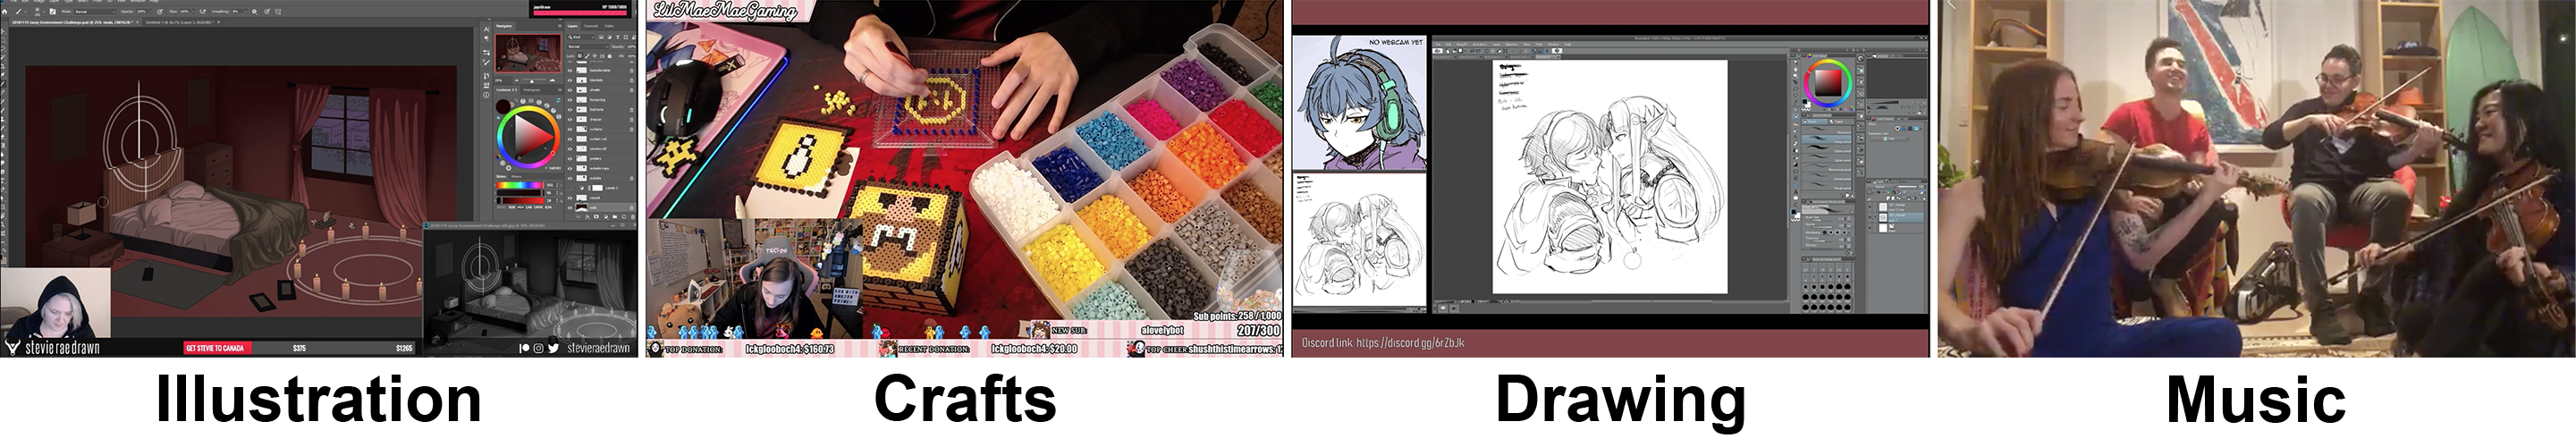
\includegraphics[width=\textwidth]{liveclips/figures/examples-horizontal.png}
  \caption{Examples of creative live streams on Twitch, YouTube, and Facebook. Artists stream videos of themselves working on creative projects. Sources for video screenshots, from left to right: \href{http://bit.ly/2SK5zWE}{\nolinkurl{bit.ly/2SK5zWE}}, \href{http://bit.ly/2Bv9Y69}{\nolinkurl{bit.ly/2Bv9Y69}}, \href{http://bit.ly/2SJYFRa}{\nolinkurl{bit.ly/2SJYFRa}}, \href{http://bit.ly/2TK12Rq}{\nolinkurl{bit.ly/2TK12Rq}}}~\label{fig:livestream_examples}
\end{figure}

This chapter introduces LiveClips, a system for automatically selecting inspirational segments from long live streamed videos and recommending them as examples to users in the context of their creative workflow. We choose to present examples inside the user's software in an effort to make examples more available throughout the entire creative process.
%based on the known benefits of contextual in-application learning \cite{Grossman2010a, Pongnumkul2011, Kelleher2005, Dontcheva2014}. 
Contextually available examples increase the likelihood of unexpected, or ``serendipitous'' discoveries, which research has shown can spark new ideas in a wide range of creative domains, such as scientific research, writing, and visual art \cite{Bawden1986, Benjamin2014, Foster2003, Erdelez1999}. LiveClips' goal is to make examples pervasive in the creative process, to promote and encourage serendipitous moments of inspiration. 

LiveClips combines telemetry and computer vision techniques to automatically segment long videos into short 25-second clips, crop clips intelligently to a thumbnail size for easy viewing, and recommend clips to creative software users based on their usage behaviour. We demonstrate LiveClips' method by using it to automatically extract and rank clips from 17 live streamed videos of artists working in two popular creative applications, Adobe Photoshop and Illustrator. We focus on digital art tasks such as design and illustration, as these are currently popular tasks for live streaming, and the software used for these tasks has wide audiences.

We compare LiveClips' ranking algorithm to human ranking and find that LiveClips is able to predict a clip's inspirational value with reasonable accuracy. To demonstrate how short inspirational clips can be contextually embedded in creative software, we present a design space and three prototypes that lie within this space, implemented in Adobe Photoshop (\autoref{fig:liveclips_photoshop}). Initial user feedback suggests that this approach is promising and warrants further study. In summary, we make the following contributions:

\begin{itemize}
\item a formative understanding of creative live streaming from the perspective of both streamers and viewers,
\item a method for extracting short (25-second) clips from long live streamed videos and cropping them to thumbnail size,
\item an approach for selecting example clips to present inside creative software based on their visual properties, the user's tool usage, and the presentation location within the software,
\item three prototype implementations in a creative application and validation of the ranking approach with human raters. 
\end{itemize}
